\section{Variational Analysis} \label{sec:variational}

In Section \ref{sec:geometric} we investigated how existing tag-match relationships to a common tag influenced the distribution of match distances.
This section, in contrast, focuses on how individual mutations and cumulative sequences of mutations affect a single tag-matching relationship.

In this work, we use a bit flip mutation operator.
This approach enables straightforward, direct comparison between metrics.
However, as a result, these analyses do not explore alternate, more semantic approaches to mutation --- especially pertinent for integer tagging schemes where a tag's integer value can be directly manipulated, for example by adding or subtracting a normally-distributed amount.\footnote{
Although not universal, use of bit flip mutation operators with integer representations is not entirely uncommon.
See e.g., \cite{downing2015intelligence}.

Additionally, in a supplementary experiment we found that the bitwise mutational operator outperforms a simple Gaussian mutation operator on the 32-vertex graph-matching task discussed in Section \ref{sec:graph-matching}.
This simple operator applies Gaussian noise to the integer value of all tags in a genome every generation; addition of an additional ``mutation probability'' parameter may yield better results.
Supplementary Section \ref{sec:graph-matching-norm} provides details on this experiment.
This finding further motivates our limitation of scope to bitwise mutations in this initial work.
}
Any extrapolation of these results to systems with different mutation operators should be made with careful consideration, and may merit additional experimentation or analysis.

In Section \ref{sec:single_step}, we report two single-step mutational analyses: one that examines the local mutational neighborhoods of loosely-affiliated tag pairs and a second that examines the local mutational neighborhoods of tightly-affiliated tag pairs.
In Section \ref{sec:mutational_walks}, we perform mutational walk analysis to survey the broader mutational landscape.

\subsection{Single-Step Mutations} \label{sec:single_step}

\begin{figure}
\begin{center}

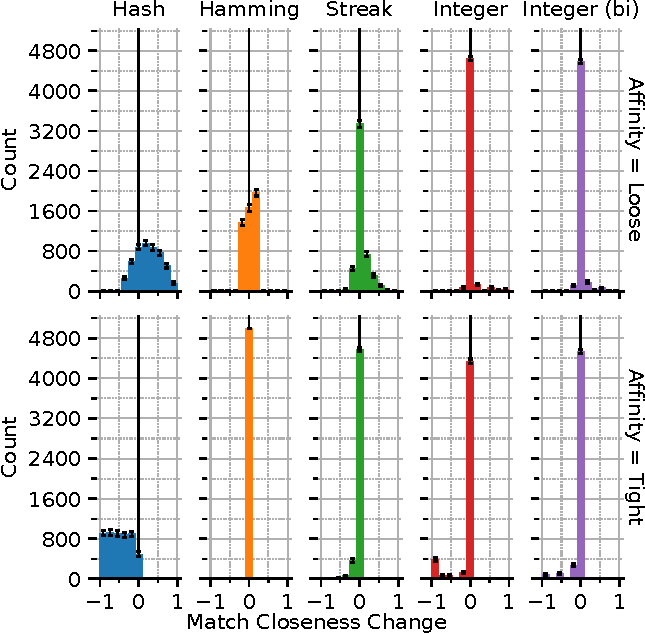
\includegraphics[width=\columnwidth]{img/mutational_step/bitweight=0dot5+seed=1+title=low-mutational-step+viz=hist+_data_hathash_hash=95a57768de56995a+_script_fullcat_hash=aa068ad24b386169+ext=}
\caption{
Distributions of mutation effects on match distance for loosely matched (pre-mutation match distance $> 0.5$) and tightly matched (pre-mutation match distance $< 0.01$) tag pairs.
Note that match closeness change (rather than mast distance change) is plotted so that better-matching mutational outcomes fall to the right and worse-matching mutational outcomes fall to the left.
Error bars are 95\% confidence intervals calculated using the Wilson score method with continuity correction \citep{newcombe1998two}.
Supplementary Figure \ref{fig:mutational_step_supp} shows the cumulative distribution of all sampled match distance changes for each metric.
}
\label{fig:mutational_step}

\end{center}
\end{figure}


We performed single-step mutational analyses to characterize the local mutational neighborhoods induced by each tag-matching metric.

To measure the effect of mutation on loosely-affiliated tag pairs, for each metric $m$ we
\begin{itemize}
    \item randomly sampled a target tag $R$,
    \item randomly sampled candidate tags until we found a second tag $S$ with a match distance $m(R, S) > 0.5$,
    \item recorded match distance between $R$ and $S$, $d = m(R, S)$,
    \item applied a one-bit mutation to the secondary tag $S$, yielding a mutated variant $S'$,
    \item measured the match distance between $R$ and $S'$, $d' = m(R, S')$,
    \item and then calculated change in match distance under mutation $p = d' - d$.
\end{itemize}
We repeated this procedure to generate 5,000 samples.

To suit the instinct that positive change should correspond to an increase in match quality and negative change should correspond to a decrease in match quality, we pose all further discussion in terms of match cloesness change rather than match distance change.

The top panel of Figure \ref{fig:mutational_step} visualizes the distribution of match closeness change under mutation of loosely-affiliated tags.
Negative match closeness change --- falling on left side of $x$-axes in Figure \ref{fig:mutational_step} --- corresponds to a decrease in match quality.
Conversly, positive match closeness change falls on the right side of $x$-axes in Figure \ref{fig:mutational_step} and denotes an increase in match quality.

We used a similar procedure to measure the distribution of mutational perturbations on tightly-matched tag pairs, except that we uniformly sampled until we found a second tag $S$ with match distance $< 0.01$.
The bottom panel of Figure \ref{fig:mutational_step} visualizes the distribution of match distance change under mutation of tightly-affiliated tags.
This distribution reflects the effects of one-step mutations on tags with pre-existing affinity.

\subsubsection{Hash Metric}

The hash metric exhibits the thickest tails of mutational magnitude of all metrics.
Extreme-effect one-step mutations are plentiful under this metric.
Interestingly, compared to other metrics, the hash metric exhibits a greater fraction of mutations that reduce affinity between tightly-affiliated tags and a greater fraction of mutations that increase affinity between loosely-affiliated tags.
This result can be attributed to the hash metric's lack of geometric structure.
Because all one-step mutations uniformly sample a new match distance, 99.5\% of one-step mutations on tightly-affiliated tags will result in a looser coupling.
Similarly, approximately 75\% of one-step mutations on loosely-affiliated tags will result in a tighter coupling.

\subsubsection{Hamming Metric}

The Hamming metric consistently exhibits small-magnitude match-closeness changes under mutation.
High-magnitude one-step mutations do not occur under this metric.
(Without normalizing match distance to a uniform distribution for randomly-sampled tags, all Hamming metric mutations would be of exactly the same magnitude, either increasing or decreasing the count of matching bits by 1.)

\subsubsection{Streak Metric}

Unlike all other metrics, the streak metric frequently yields perfectly neutral outcomes under mutation.
With loose affinity, 56\% of all mutations were perfectly neutral.
With tight affinity, 45\% of all mutations were perfectly neutral.
These perfectly-neutral mutations presumably affect regions of the bitstring involved in neither the longest-matching streak nor the longest-mismatching streak.
The streak metric exhibits a thicker tail of mutational magnitude for mutations that couple loosely-affiliated tags than the integer metrics.
In addition, the most extreme mutational outcomes that couple loosely-affiliated tags appear to be of a comparable magnitude to those under the integer metrics and the Hamming metric.
Mechanistically, this might be due to mutations that disrupt longest-mismatching streaks.
However, one-step mutations that decouple tightly-affiliated tags do not appear as potent.
This might be because achieving a very poor match requires both increasing longest-mismatching streak length and decreasing longest-matching streak length.

\subsubsection{Integer and Bidirectional Integer Metrics}

For both tightly- and loosely-affiliated tag pairs under the integer and bidirectional integer metrics, most mutations caused very small changes in match closeness.
These mutations toggle less-significant bits of the tag's integer representation.
However, under these metrics, a small fraction of mutations affecting more-significant bits of the integer representation have a much stronger effect.
Single-step mutations occasionally occurred that conspicuously couple loosely-affiliated tag pairs or conspicuously decouple tightly-affiliated tag pairs.
For instance, under the integer metric 3.6\% of mutations increased loosely-affiliated match closeness by at least 0.25 units and and 10.6\% decreased tightly-affiliated match closeness by at least 0.25 units.
Under the bidirectional integer metric, these percentages were 3.3\% and 3.9\%, respectively.
Notably, the unidirectional integer metric exhibits more frequent strong decoupling mutations than the bidirectional integer metric, presumably due to its non-commutative quirks.

\subsection{Mutational Walks} \label{sec:mutational_walks}

\begin{figure}
\begin{center}

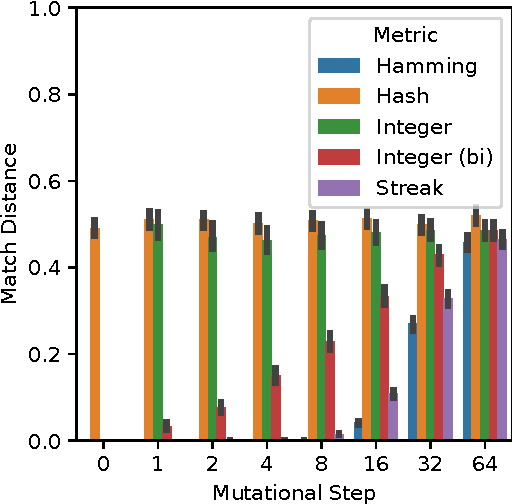
\includegraphics[width=\columnwidth]{{{mutational_walk/bitweight=0.5+seed=1+title=mutational_walk_barplot+_data_hathash_hash=8bf152d87daa9cb7+_script_fullcat_hash=982405ca713eba73+ext=}}}
\caption{
Snapshots of match distance at exponentially increasing steps from identical tags.
Error bars represent 95\% confidence intervals.
}
\label{fig:mutational_walk_barplot}

\end{center}
\end{figure}


We performed multi-step mutational analyses to characterize the broader mutational landscapes induced by each tag-matching metric.
To conduct these mutational walks, for each metric $m$ we
\begin{itemize}
    \item randomly generated a starting tag $t^{(0)}$,
    \item then sequentially applied randomly-chosen one-step bit flip mutations to that tag until a mutational saturation threshold (yielding a sequence of tags $t^{(1)}, t^{(2)}, ...$),
    \item while recording match distance from the original starting tag $m(t^{(0)}, t^{(i)})$ at each step $i$ along the walk.
\end{itemize}
Back mutation was allowed in these experiments.
We performed 65 step mutational walks, which allowed us to cover one binary order of magnitude past one expected mutation per site at 32 steps.
We analyzed 1,000 replicate mutational walks for each metric, which was sufficient to distinguish metrics with bootstrapped 95\% confidence intervals

Figure \ref{fig:mutational_walk_barplot} shows how match distance increases along mutational walks for each tag-matching metric.

\subsubsection{Hash Metric}

Due to the hash metric's lack of geometric structure, bitwise equivalent tags do not exhibit low match distance.
So, as expected, throughout the entire mutational walk this metric maintains a constant mean match distance of 0.5.

\subsubsection{Hamming Metric}

The Hamming metric's match distance diffuses upward slowest.
The Hamming metric's mutational walk is significantly slower to diverge than the streak metric's at 16 and 32 steps (non-overlapping 95\% CI).
It is significantly slower to diverge than the integer metrics and the hash metric between steps 1 and 32, as well (non-overlapping 95\% CI).

\subsubsection{Streak Metric}

The streak metric diffuses away from zero match distance second-slowest, trailed only by the Hamming metric.

Interestingly, this result contradicts Downing's presentation of the streak metric in \citep{downing2015intelligence}, in which he suggests that the streak metric exhibits \textit{greater} robustness because its match distance diverges more slowly under a mutational walk.
This discrepancy presumably arises due to our uniformification to ensure a uniform distribution of raw match scores between 0 and 1 (Section \ref{sec:uniformification}).
We believe that our result under uniformification is more representative because match distance corresponds to the probability that arbitrary tags would match more strongly by chance --- which directly relates to how effectively a operand tag competes to be the ``best'' match for a query.

To compare mutational landscapes between the streak and integer metrics under more realistic circumstances (i.e., where tags do not begin exactly perfectly-matched), we performed a secondary mutational walk experiment.
This experiment was conducted exactly as before, except instead of starting with exactly-identical tags it started with a pair of tags that was randomly sampled for match distance $<0.01$.

As shown in Supplementary Figure \ref{fig:mutational_walk_sampled_start_barplot}, this experiment confirmed greater robustness of the Hamming metric under mutation.
The streak metric's match distance was significantly greater than the Hamming metric between mutational steps 2 and 16 (non-overlapping 95\% CI).
Our result remained consistent when replicating the experiment with 64-bit tags (Supplementary Figure \ref{fig:mutational_walk_sampled_start_64_barplot}).

\subsubsection{Integer Metric and Bidirectional Integer Metric}
\label{sec:mutation_integer}

The binary representation of the integer and bidirectional integer metrics (Section \ref{sec:integer}) induces a long-tailed distribution of mutational effect sizes.
Under this distribution, value changes of each binary order of magnitude are equally likely (corresponding to toggling the bit at each position).
Occasional large-effect mutations provide plausible explanation for the bidirectional integer metric's rapid increase in match distance under mutation relative to the Hamming and streak metrics.
The integer metric experiences even more rapid dilation of match distance under mutation.
Under this metric, half of first mutational steps cause a wraparound effect, immediately spiking the average match distance to 0.5.
Supplementary Figure \ref{fig:mutational_walk_lineplot} shows match distance variance decreasing as the integer metric mutational walk proceeds away from match distances biased to 0 or 1.
